%From diagram \ref{fig:diagramSystem}, my system has four main blocks. This chapter is dedicated to describe functionalities of these components as well as the background behind.
This chapter is dedicated to describe briefly theoretical background as well as alternative solutions to subtasks of the project. We will cover from automatic Speech-To-Text, Information Extraction, to Deep Convolutional Neural Network to classify image etc.

\section{Automatic Speech Recognition system}
Automatic Speech Recognition (ASR) system is the core part in any voice command system. Given the audio input, ASR system will output the text form of the input for later processing. Briefly, the audio input is in form of a sound wave over the recording time. It's sampled at a rate of 16000Hz which is enough for recognition. Then this sound wave is chunked at each 20ms and transformed to a spectrogram by using Fourier transform. This then be feeded to a kind of recurrent neural network \cite{Medium:2016}. The output at each time slot is the characters and we normally have a language model to refine this. 

Note that to build an ASR system that performs at the level of Amazon Alexa or Google Now, we need a lot of training data in both quantity (hundreds of thousands hours of spoken audio) and diversity (native and non-native speakers, with and without background noise, etc.) And this kind of data is not available. As the main objective of the project is to use voice to control the robot, not to build a decent ASR system hence I decided to use existing softwares. I explored two solutions: open source systems and Google Cloud.

\subsection{Open-source ASR}
I tried several open-source softwares such as Kaldi \cite{Kaldi:2017}, CMUSphinx \cite{CMUSphinx:2017} and Deep Speech Nervana \cite{DeepSpeech:2017}. As a non-native speaker, I found that they do not perform at an adequate level. For example, I often get "tune rite" when I say "turn right". In addition, it's not easy to use the libraries because long installation processes are required and proper documentations of their usage are limited.

\subsection{Google Cloud Speech API}
My alternative solution is to use a cloud service Google Speech API \cite{GoogleCloud:2017}. Although the system needs to have internet access, it provides qualitative speech recognition and easy to use: we send the audio content and get back the text. By this, we also cut the computation cost of using an ASR server locally. Note that state of the art ASR systems use deep neural network which requires massive computations and resources. For those reasons, I chose to use Google Speech API in my system.

\section{Neural Network Overview}
Neural network is a key technique behind many artifical intelligent systems today. There were already a lot of research about neural network in late 20th century. However, this method only dominates other methods recently (around 2012) thanks to the availability of large datasets and the capability of powerful computation units (GPUs). This section presents briefly convolutional neural networks which is used to classify image.
\subsection{Fully-connected Neural Network}
A fully connected neural network is a directed graph composed by a input layer, several hidden layers and an output layer. An example is shown in figure \ref{fig:fcNet}: The input data is presented by the input layer (e.g. vector of features of input) and is feeded forward through the network to the output layer which represents the probabilities of input's labels. Between each layers, there are learnable parameters: matrix \textbf{weight $W$} and vector \textbf{bias $b$}. Based on the dimensions of input features, number of classes, and hidden layers' sizes, we can easily determine the dimension of these parameters. 
\begin{figure}[tb]
	\centering
	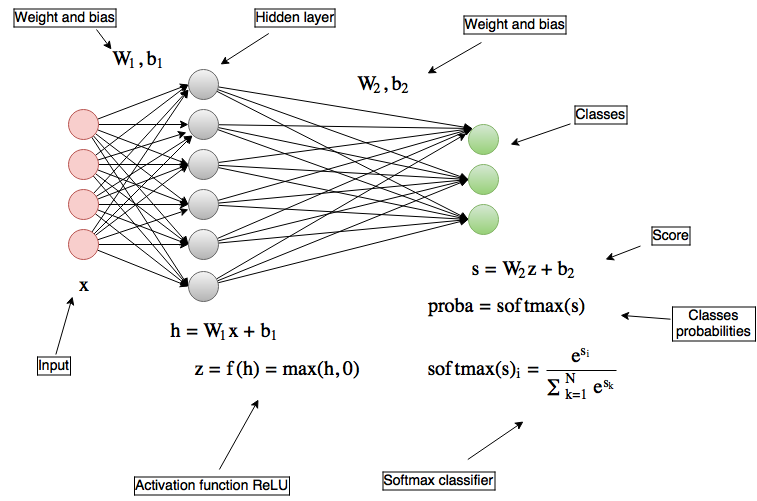
\includegraphics[width=0.9\hsize]{./figures/fcNet}
	\caption{A simple fully connected neural network which classifies an input data into 3 categories using softmax classifier and rectified linear unit activation function (ReLU).}
	\label{fig:fcNet}
\end{figure}
In practice, fully-connected layers are combined with other blocks and they are usually the final block of a classification model. For example, figure \ref{fig:convNet1} shows a simple convolutional neural network with fully-connected layer at the end to classify the input image.
\begin{figure}[tb]
	\centering
	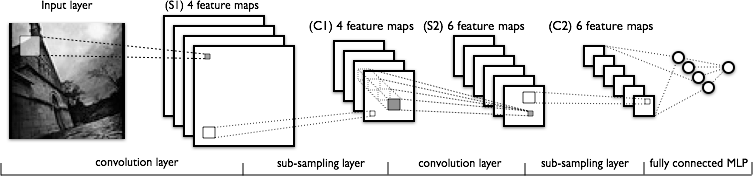
\includegraphics[width=0.9\hsize]{./figures/convNet1}
	\caption{A simple convolutional neural network: its neurons are transposed into 3D shape (width, height and depth) at each layer. The fully connected layer is placed at the end to classify input.}
	\label{fig:convNet1}
\end{figure}
\subsection{Convolutional Neural Network}
Image inputs usually have a 3D shape: width, height and 3 color channels (RGB). Hence, convolutional neural network also aranges its neurons in 3 dimensions: width ($w$), height ($h$), depth ($h$). Note that the depth of input layer equals the number color channels of input image and the \textbf{depth of convolution layer equals the number of filters applied at that layer}. If we use filters of size $3*3$, then in a convolutional layer $i$:
\begin{itemize}
	\item the weight $W_i$ is a stack of filters and $dim(W_i) = 3*3*d_{i-1}*d_i$ where $d_{i-1}$, $d_i$ are depth of layer $i-1$ and $i$ respectively.
	\item the bias $b_i$ is the vector with length equals number of filters, i.e. $b_i \in R^{d_i}$
	\item We convolve the tensor input $w_{i-1}*h_{i-1}*d_{i-1}$ coming from layer $i-1$ with a filter block $3*3*d_{i-1}*d_{i}$ to obtain tensor size $w_{i-1}*h_{i-1}*d_{i}$. Note that we convolve with padding input to keep the same width and height dimension after convolving.
	\item We add bias $b_i$ element-wise for each "surface" (or "slice") $w_{i-1}*h_{i-1}$ of the current tensor.
	\item We apply activation function ReLU to current tensor.
	\item We sub-sample the current tensor to keep strongest features and reduce tensor size. We have final output tensor of size $w_i * h_i *d_i$
\end{itemize}  
The process is illustrated in figure \ref{fig:convNetsimple}. And a common method for sub-sampling called \tbf{max-pooling} shown in figure \ref{fig:maxpool}. It partitions each "slice" of the tensor into non-overlapping rectangles and choose the maximum value in each rectangle. Hence, we produce non-linearities and prioritise strongest features.
\begin{figure}[tb]
	\centering
	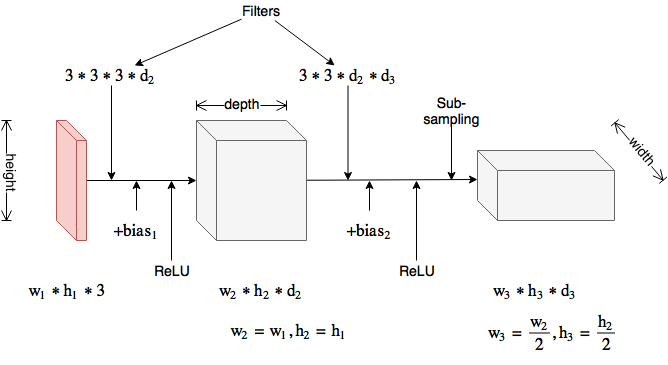
\includegraphics[width=0.9\hsize]{./figures/convNetsimple}
	\caption{Operations and parameters of convolution layers. Note that only input image and 2 convolution layers are drawn here.}
	\label{fig:convNetsimple}
\end{figure}
\begin{figure}[tb]
	\centering
	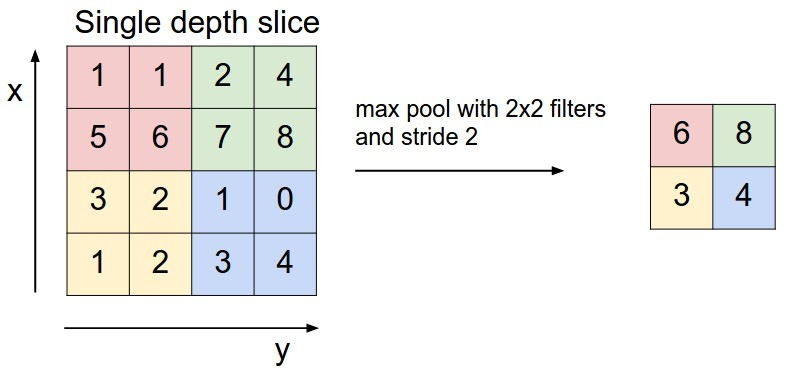
\includegraphics[width=0.6\hsize]{./figures/maxpool}
	\caption{Max-pooling to reduce tensor size and keep strongest features.}
	\label{fig:maxpool}
\end{figure}

After several convolution layers, we flatten the tensor to put into a fully connected neural network for classification. Note that at these fully connected layers, we often use \textbf{dropout} which is a technique to reduce overfitting at fully connected layers because most of parameters present at these layers (figure \ref{fig:dropout}). In training time, we have a probability (normally $p=0.5$) of dropping out neurons in the fully connected layers from the network and then reinsert the dropped out nodes. We repeat that process for every forward and ackward pass. This will also bring a similar effect as model ensemble. In addition, dropout technique can also be used at convolution layers. For more detail about dropout, please refer to \cite{Srivastava:2014:DSW:2627435.2670313}.
\begin{figure}[tb]
	\centering
	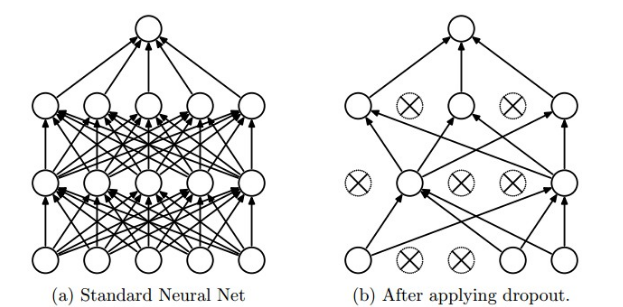
\includegraphics[width=0.8\hsize]{./figures/dropout}
	\caption{Dropout helps to reduce overfitting and ensemble models. Image taken from original paper \cite{Srivastava:2014:DSW:2627435.2670313}.}
	\label{fig:dropout}
\end{figure}

\subsection{Loss Function}
We are left to define a loss function: which allows us to train a machine learning model by updating parameters in order to minimise loss. For classification problems we often use the popular cross-entropy loss function. Consider an input indexed $i$, then its cross-entropy loss is
\begin{align}
\label{form:CELoss}
L_i(s) = -\log(\frac{e^{s_{y_i}}}{\sum_{k=1}^{N}e^{s_k}}) = -s_{y_i} + \log\sum_{k=1}^{N}e^{s_k}
\end{align}
where $y_i$ is its ground-truth label, and $s$ denotes its score at the last layer (see figure \ref{fig:fcNet}). We can see from formula \ref{form:CELoss} that if the score for ground-truth label gets bigger then the loss gets smaller.

Now, given the loss function, we will use stochastic gradient descent to minimise it. There is one hyperparameter related to this optimisation technique which is the learning rate.

\subsection{Train, validate and test}
To train and validate a machine learning model, we usually split the dataset into 3 parts: training set ($\approx56\%$), validation set ($\approx14\%$) and test set ($\approx30\%$). We will use training dataset to train the model (in our case they are all the parameters $W_i$, $b_i$) and use the validation dataset to tune other hyperparameters: learning rates, dropout probability, hidden layer sizes, number of filters etc. Once we have done our best on the validation set, we run a run the model only once on the test dataset and obtain the test accuracy. This figure will be our model performance. 

\section{Image Classification}
\subsection{Overview}
\textbf{Image Classification} is the task of assigning an input image to one label from a fixed set of categories. It's directly related to our object finding problem and we need to solve this first. However, in reality, we are likely to have input image that can contain several objects at once. The related problems are named \textbf{Object Detection} and \textbf{Segmentation}. Image Classification is needed to solve those problems and particularly, if the robot takes images at different view, there might exist the case where only one object is captured and the problem reduces to classify the image. This is not to say that the Image Classification is an easy task. By contrast, this is really hard problem given the following challenges (figure \ref{fig:ImClasschallenges}):
\begin{enumerate}
	\item Viewpoint variation: the same object can be captured at different camera pose.
	\item Illumination conditions: computers only see the pixel values and minor changes in illumination can result in totally different pixel values. 
	\item Scale variation: the same object can have different sizes in the real world. In addition, the distance of taking photo also cause this variation.
	\item Deformation: many objects are not static hence theirs forms are never unique.
	\item Occlusion: depend on the camera view, sometime only a portion of object is visible.
	\item Background clutter: when object and background are similar
	\item intra-class variation: there are many different types and styles of the same object class (e.g. keys, chairs)
\end{enumerate}

\begin{figure}[tb]
\centering
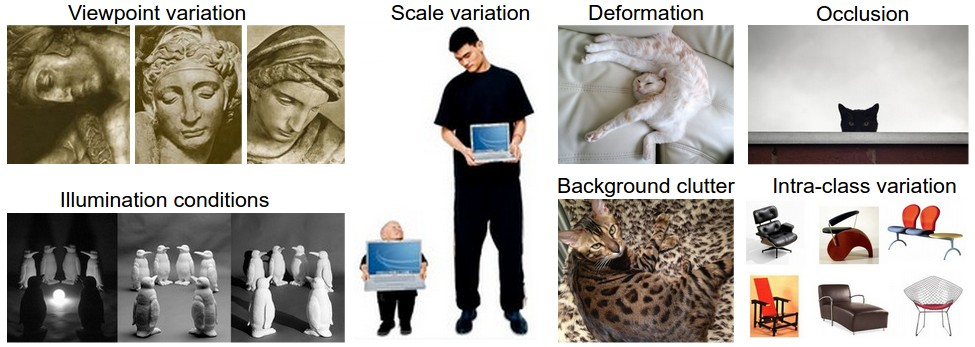
\includegraphics[width =0.9\hsize]{./figures/ImClasschallenges}
\caption{Some challenges of Image Classification problem}
\label{fig:ImClasschallenges}
\end{figure}
\subsection{State-of-the-art Solution}
The family of the best solutions for image classification up to now is deep convolutional neural networks (CNN). Figure \ref{fig:imagenetTop5Err} illustrates this point. Below are some brief explaination for its success:
\begin{itemize}
	\item Deep neural networks accomodate non-linearity properties through activation layers. This makes the system more flexible and able to prioritise important features.
	\item Each convolutional layer is a stack of filters. After learning (i.e. at test time), those filters can extract from input image many types of features such as: edge, shape, colors etc. (for more details see \cite{DeepVis:2015})
	\item Convolutional layers act as features builder, and given enough data, machines do this job better than a human (figure \ref{fig:imagenetTop5Err}).
\end{itemize}


\begin{figure}[tb]
\centering
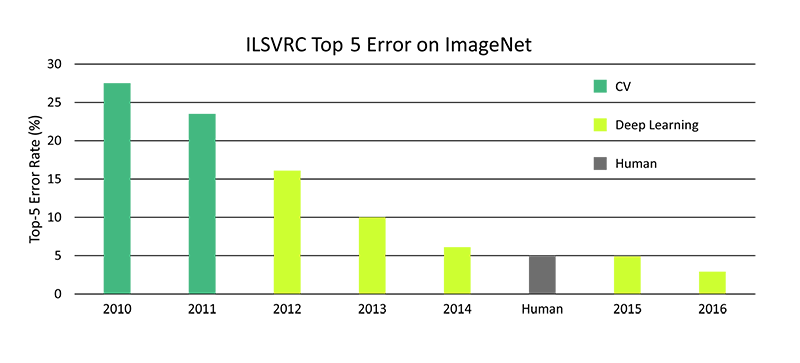
\includegraphics[width=0.9\hsize]{./figures/imagenetTop5Err}
\caption{Top 5 error rate in Imagenet Classification competition from 2010 to 2016. We can note a huge improvement from traditional approaches which use hand-crafted computer vision classifiers (CV) to deep convolutional neural network. VGG model \cite{DBLP:journals/corr/SimonyanZ14a} is the winner in 2014. Its performance nearly equals to human beings.}
\label{fig:imagenetTop5Err}
\end{figure}

\subsection{Transfer Learning from VGG16 model}
To solve my classification problem, I propose to use the VGG16 model \cite{DBLP:journals/corr/SimonyanZ14a} with some modifications at the fully connected layers as we do not have to classify 1000 objects. The original VGG16 model is illustrated in figure \ref{fig:originalVgg16}. Two reasons of using VGG16 model are its good performance and its simplicity compared to other successful models (Microsoft ResNet \cite{DBLP:journals/corr/HeZRS15}, Google Inception \cite{DBLP:journals/corr/SzegedyVISW15}, etc.)
\begin{figure}[tb]
	\centering
	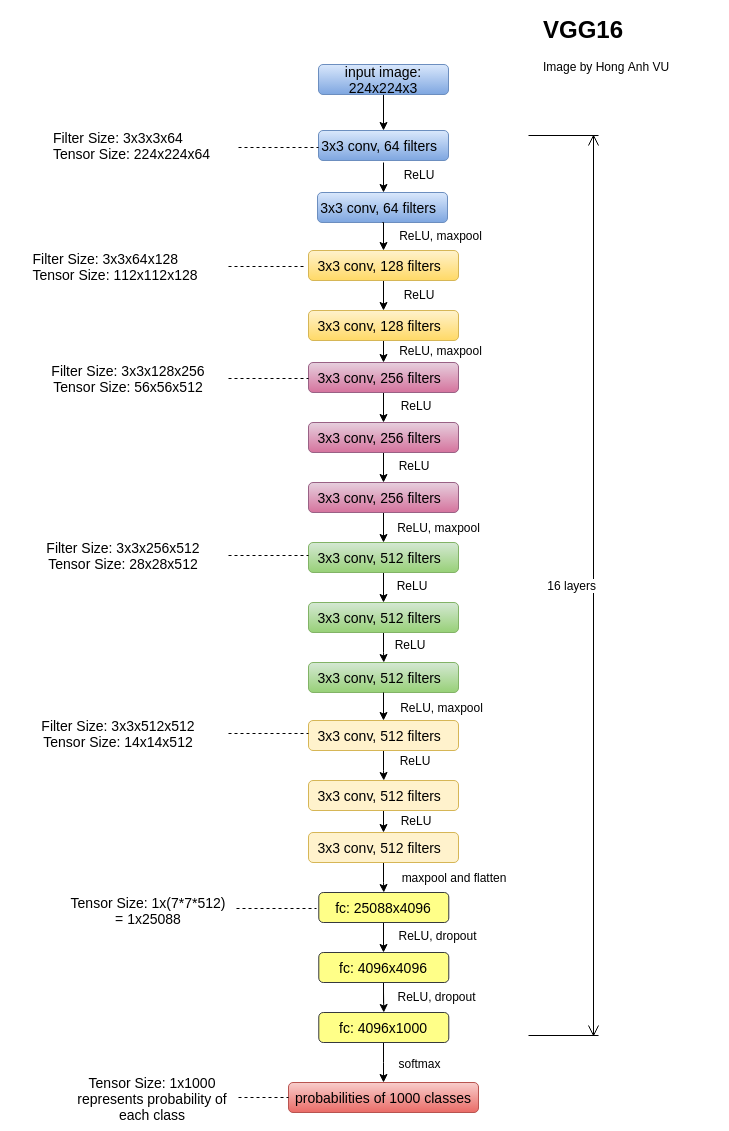
\includegraphics[width=0.9\hsize]{./figures/originalVgg16}
	\caption{Original VGG16 model}
	\label{fig:originalVgg16}
\end{figure}

In my object finding problem, I propose to classify about 12 categories: "apple", "pen", "book", "monitor", "mouse", "wallet", "keyboard", "banana", "key", "mug", "pear", "orange". They are ordinary objects that we see and use daily. To form the dataset, I downloaded 1200 images for each category from ImageNet \cite{imagenet_cvpr09}. In order to solve my problem, I use pretrained weights of convolution layers from original VGG16 model \cite{WeightsVGG:2016} and modify and retrain the fully connected layers (figure \ref{fig:transferedVgg16}). Currently, I obtained a $\approx88\%$ accuracy on test set.
\begin{figure}[tb]
	\centering
	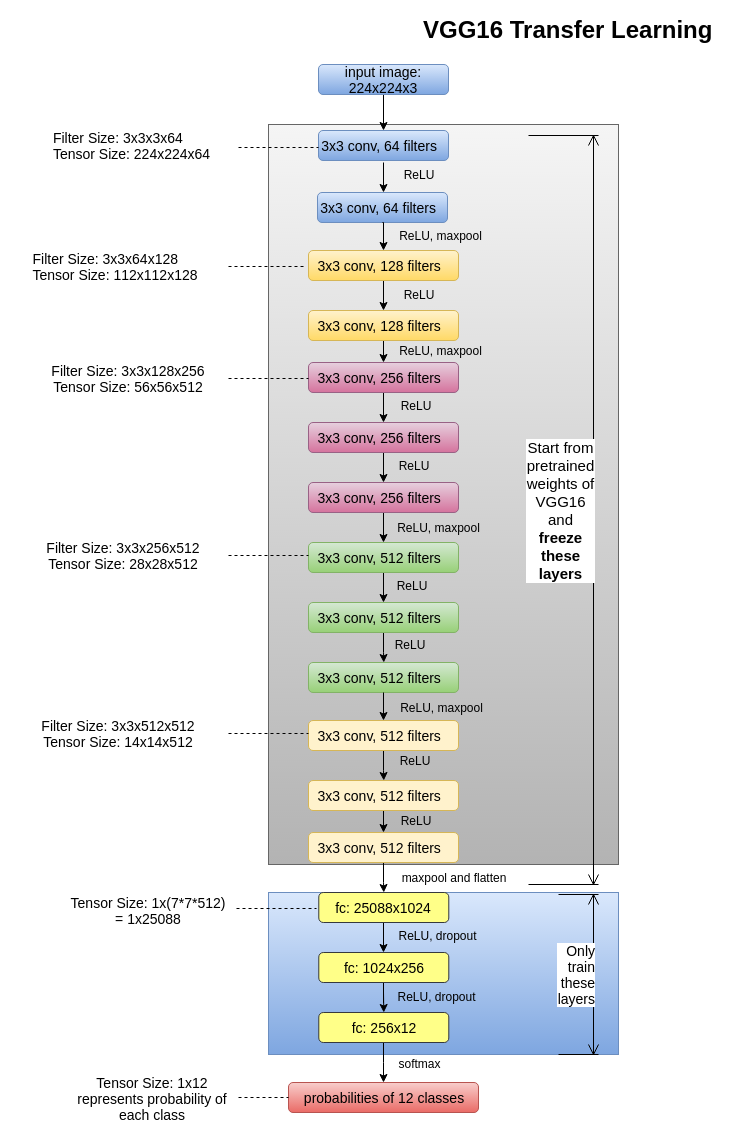
\includegraphics[width=0.9\hsize]{./figures/transferedVgg16}
	\caption{Transfer Learning from VGG16 model}
	\label{fig:transferedVgg16}
\end{figure}
